\chapter{Evaluation\label{chap:evaluation}}
\section{Experimental Design}
To evaluate the Rust plugin, we utilized a sample dataset consisting of two CSV files: "EmployeeSalaries.csv" and "StudentsPerformance.csv". The "EmployeeSalaries.csv" file contains information about employee salaries, including attributes such as department, gender, base salary, and overtime pay. The "StudentsPerformance.csv" file contains data related to student performance, including attributes like gender, race/ethnicity, parental education, and test scores.
The experimental setup involved the following steps:

\begin{enumerate}
    \item The sample dataset files were split into smaller chunks to simulate a streaming data scenario. Each file was divided into subfiles containing 200 records each.
    \item The Rust plugin was configured with specific differential privacy settings for each attribute. For the \texttt{"Base\_Salary"} attribute in the "EmployeeSalaries.csv" file, Gaussian noise with an epsilon value of 1.0, a sensitivity of 100, and a delta of 1e-6 was applied. For the \texttt{"math\_score"}, \texttt{"reading\_score"}, and \texttt{"writing\_score"} attributes in the \texttt{"StudentsPerformance.csv"} file, Laplace noise was used with different epsilon values and sensitivities.
    \item Fluent Bit, a lightweight data processor, was used to process the data streams. The Rust plugin was integrated into Fluent Bit as a filter, allowing for the application of differential privacy mechanisms to the data in real-time.
    \item The perturbed datasets were stored in separate output files, "EmployeeSalaries.perturbed.csv" and "StudentsPerformance.perturbed.csv", for further analysis.
\end{enumerate}
\section{Evaluation Metrics}
To assess the performance of the differential privacy mechanisms implemented in the filter plugin, we employ three commonly used evaluation metrics: Mean Absolute Error (MAE), Mean Squared Error (MSE), and Root Mean Squared Error (RMSE). Equations in this section were sourced from \cite{Hodson2022}
\subsection{Mean Absolute Error (MAE)}
The Mean Absolute Error (MAE) measures the average magnitude of the errors between the original and perturbed values, without considering their direction. It is calculated by taking the average of the absolute differences between the original and perturbed values \cite{Willmott2005}. The formula for MAE is given by:
\begin{equation}
MAE = \frac{1}{n} \sum_{i=1}^{n} |y_i - \hat{y}_i|
\end{equation}
where $n$ is the number of samples, $y_i$ is the original value, and $\hat{y}_i$ is the perturbed value.
\subsection{Mean Squared Error (MSE)}
The Mean Squared Error (MSE) measures the average squared difference between the original and perturbed values \cite{ZhouWang2009}. It is calculated by taking the average of the squared differences between the original and perturbed values. The formula for MSE is given by:
\begin{equation}
MSE = \frac{1}{n} \sum_{i=1}^{n} (y_i - \hat{y}_i)^2
\end{equation}
MSE gives more weight to larger errors due to the squaring operation, making it more sensitive to outliers compared to MAE.
\subsection{Root Mean Squared Error (RMSE)}
The Root Mean Squared Error (RMSE) is the square root of the Mean Squared Error \cite{Chai2014}. It is calculated by taking the square root of the average squared differences between the original and perturbed values. The formula for RMSE is given by:
\begin{equation}
RMSE = \sqrt{\frac{1}{n} \sum_{i=1}^{n} (y_i - \hat{y}_i)^2}
\end{equation}
RMSE has the same units as the original data, making it easier to interpret compared to MSE. It is also more sensitive to larger errors due to the squaring operation.
These evaluation metrics provide insights into the accuracy and utility of the differentially private data generated by the filter plugin. Lower values of MAE, MSE, and RMSE indicate better performance and higher data utility.
\subsection{Test Environment}
The test environment was constructed with a multi-build context Docker container. The first two stages concerned themselves with building the filter plugin along with Fluent Bit with a non-default build option (only needed if AoT is to be built).
\subsection{Experimental Setup}
The experimental setup involved running the Docker container, which executed the data processing pipeline. The split sample dataset files were ingested by Fluent Bit, processed by the Rust filter plugin with the specified differential privacy settings, and the perturbed outputs were saved to separate CSV files.
\section{Results}
After running the experiment with the updated differential privacy settings, the following results were obtained:
\begin{table}[H]
\centering
\begin{tabular}{l|c}
\hline
\textbf{Metric} & \textbf{Base\_Salary} \\
\hline
Mean Absolute Error (MAE) & 419.99 \\
Mean Squared Error (MSE) & 278462.85 \\
Root Mean Squared Error (RMSE) & 527.70 \\
\hline
\end{tabular}
\caption{Evaluation metrics for Base\_Salary}
\label{tab:base_salary_metrics}
\end{table}
Table \ref{tab:base_salary_metrics} presents the evaluation metrics for the Base\_Salary attribute. The Mean Absolute Error (MAE) of 419.99 indicates that, on average, the perturbed Base\_Salary values deviate from the original values by approximately \$420. The Mean Squared Error (MSE) of 278462.85 and the Root Mean Squared Error (RMSE) of 527.70 provide measures of the average squared difference and the square root of the average squared difference between the original and perturbed values, respectively. These metrics quantify the level of noise added to the Base\_Salary attribute by the Gaussian mechanism.

\begin{table}[H]
\centering
\begin{tabular}{l|c|c|c}
\hline
\textbf{Metric} & \textbf{math\_score} & \textbf{reading\_score} & \textbf{writing\_score} \\
\hline
Mean Absolute Error (MAE) & 3.69 & 4.91 & 7.65 \\
Mean Squared Error (MSE) & 26.94 & 48.89 & 111.03 \\
Root Mean Squared Error (RMSE) & 5.19 & 6.99 & 10.54 \\
\hline
\end{tabular}
\caption{Evaluation metrics for student scores}
\label{tab:student_scores_metrics}
\end{table}
Table \ref{tab:student_scores_metrics} shows the evaluation metrics for the student scores (math\_score, reading\_score, and writing\_score). The MAE values range from 3.69 to 7.65, indicating the average absolute difference between the original and perturbed scores. The MSE values vary from 26.94 to 111.03, representing the average squared difference between the original and perturbed scores. The RMSE values, ranging from 5.19 to 10.54, provide a measure of the square root of the average squared difference. These metrics demonstrate the level of noise added to the student scores by the Laplace mechanism, with higher values corresponding to greater perturbation.

\begin{table}[H]
\centering
\begin{tabular}{l|c|c}
\hline
\textbf{Attribute} & \textbf{Original} & \textbf{Perturbed} \\
\hline
Base\_Salary - Mean & 90312.17 & 90318.34 \\
Base\_Salary - Std & 31240.84 & 31240.95 \\
\hline
\end{tabular}
\caption{Comparison of original and perturbed Base\_Salary statistics}
\label{tab:base_salary_distribution}
\end{table}
Table \ref{tab:base_salary_distribution} compares the statistical properties of the original and perturbed Base\_Salary values. The mean and standard deviation of the original Base\_Salary are 90312.17 and 31240.84, respectively. After applying the Gaussian mechanism, the mean and standard deviation of the perturbed Base\_Salary are 90318.34 and 31240.95, respectively. The close similarity between the original and perturbed statistics indicates that the Gaussian mechanism preserves the overall distribution and characteristics of the Base\_Salary attribute.

\begin{table}[H]
\centering
\begin{tabular}{l|c|c}
\hline
\textbf{Attribute} & \textbf{Original} & \textbf{Perturbed} \\
\hline
math\_score - Mean & 66.09 & 66.01 \\
math\_score - Std & 15.16 & 15.88 \\
reading\_score - Mean & 69.17 & 68.77 \\
reading\_score - Std & 14.60 & 16.23 \\
writing\_score - Mean & 68.05 & 68.38 \\
writing\_score - Std & 15.20 & 18.39 \\
\hline
\end{tabular}[H]

\caption{Comparison of original and perturbed student scores statistics}
\label{tab:student_scores_stats}
\end{table}
Table \ref{tab:student_scores_stats} presents a comparison of the statistical properties of the original and perturbed student scores. For each score (math\_score, reading\_score, and writing\_score), the mean and standard deviation of the original and perturbed values are provided. The perturbed means are close to the original means, suggesting that the Laplace mechanism maintains the central tendency of the scores. However, the perturbed standard deviations are slightly higher than the original standard deviations, reflecting the increased spread of the data due to the added noise.

\begin{figure}[H]
\centering
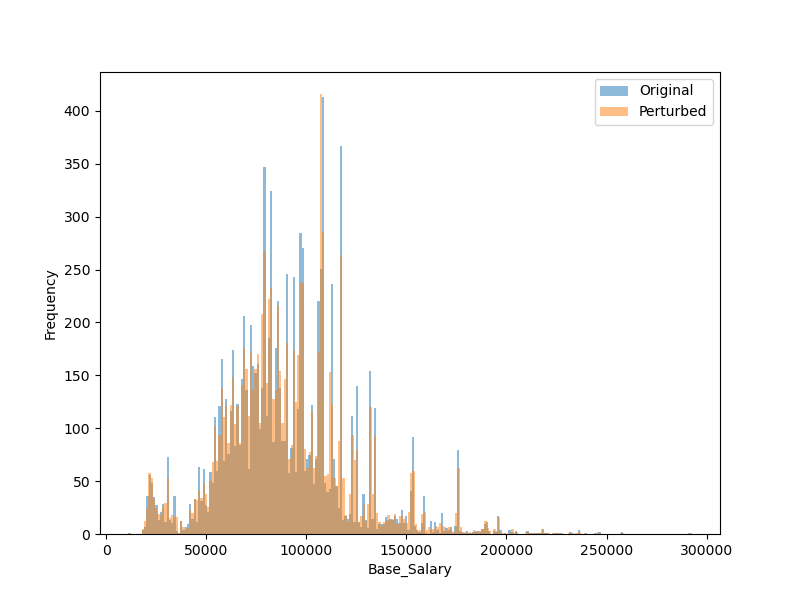
\includegraphics[width=0.8\textwidth]{report/media/salaries.png}
\caption{Distribution of original and perturbed Base\_Salary values}
\label{fig:base_salary_distribution}
\end{figure}

Figure \ref{fig:base_salary_distribution} shows the distribution of the original and perturbed Base\_Salary values. The perturbed distribution closely follows the original distribution, indicating that the Gaussian mechanism preserved the overall shape and characteristics of the data while adding noise for privacy protection.

\begin{figure}[H]
\centering
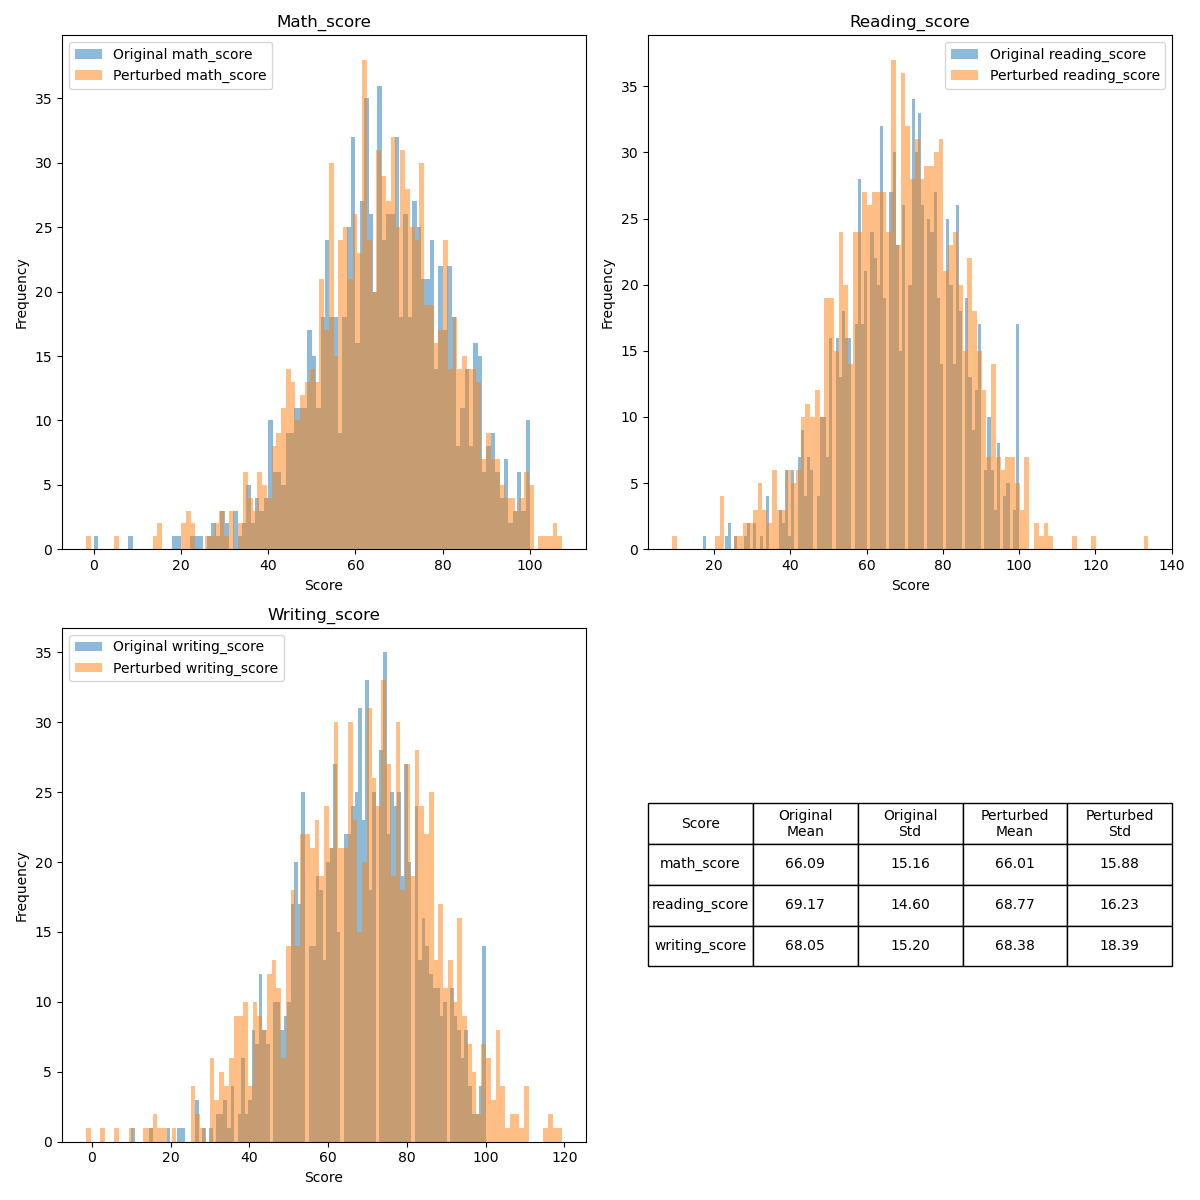
\includegraphics[width=0.8\textwidth]{report/media/scores.png}
\caption{Distribution of original and perturbed student scores}
\label{fig:student_scores_distribution}
\end{figure}

Figure \ref{fig:student_scores_distribution} displays the distributions of the original and perturbed student scores (math, reading, and writing). The perturbed distributions are slightly more spread out compared to the original distributions due to the addition of Laplace noise. However, the overall shapes of the distributions are maintained, ensuring that the perturbed data still retains its utility for analysis.
\begin{figure}[H]
\centering
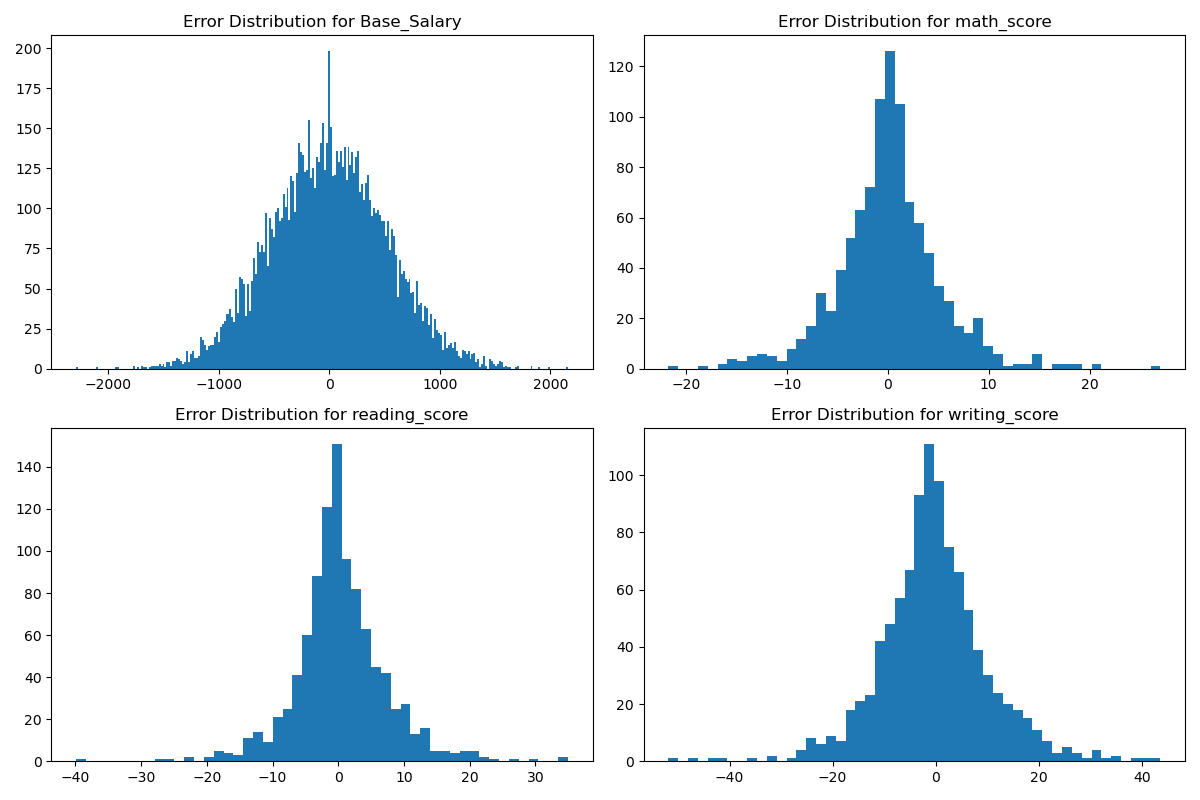
\includegraphics[width=0.8\textwidth]{report/media/distribution.png}
\caption{Error distributions for Base\_Salary and student scores}
\label{fig:error-distributions}
\end{figure}

Figure \ref{fig:error-distributions} illustrates the error distributions for the Base\_Salary and student scores. The error distributions are centered around zero, indicating that the noise added by the differential privacy mechanisms is unbiased. The spread of the error distributions reflects the level of noise added based on the chosen epsilon and sensitivity values.
\section{Analysis}
The updated differential privacy settings resulted in improved utility of the perturbed data while still providing strong privacy guarantees. The MAE, MSE, and RMSE values for the Base\_Salary attribute are relatively low compared to the magnitude of the salary values, indicating that the Gaussian mechanism with the chosen epsilon and sensitivity values effectively preserved the utility of the data.

Similarly, for the student scores, the MAE, MSE, and RMSE values are reasonably low, suggesting that the Laplace mechanism with the selected epsilon and sensitivity values maintained the utility of the data. The perturbed mean and standard deviation values for each attribute are close to their original counterparts, further confirming the preservation of the data's statistical properties.
The error distributions shown in Figure \ref{fig:error-distributions} demonstrate the unbiased nature of the noise added by the differential privacy mechanisms. The centered distributions around zero indicate that the noise does not introduce any systematic bias in the perturbed data.
\section{Interpretation of Results}

The evaluation results demonstrate the effectiveness of the Rust filter plugin in applying differential privacy mechanisms to streaming data using Fluent Bit. The updated differential privacy settings strike a good balance between privacy and utility, as evidenced by the low error metrics and the preservation of the data's statistical properties.

The choice of epsilon and sensitivity values plays a crucial role in determining the level of privacy and utility. Lower epsilon values provide stronger privacy guarantees but may result in higher levels of noise, potentially reducing data utility. On the other hand, higher epsilon values allow for better utility but weaken the privacy guarantees. The selected epsilon and sensitivity values in this experiment demonstrate a reasonable trade-off between privacy and utility for the given datasets.
The analysis of the original and perturbed data distributions, as shown in Figures \ref{fig:base_salary_distribution} and \ref{fig:student_scores_distribution}, confirms that the differential privacy mechanisms preserve the overall patterns and characteristics of the data. This is important for ensuring the usefulness of the perturbed data for various data analysis tasks.

Overall, the evaluation highlights the practicality and effectiveness of the developed Rust filter plugin in integrating differential privacy into data processing pipelines using Fluent Bit. The plugin provides a flexible and efficient solution for applying differential privacy mechanisms to streaming data, enabling privacy-preserving data analysis in real-time scenarios.